\begin{figure}
\centering
\begin{subfigure}{0.31\textwidth}
    \centering
    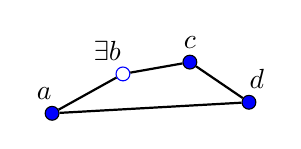
\begin{tikzpicture}
        \node[draw, circle, black, fill=blue, inner sep=0pt, minimum size=5pt,label={[xshift=-0.1cm, yshift=-0.05cm]$a$}] (a) at (0,0) {};
        \node[draw, circle, blue,  inner sep=0pt, minimum size=5pt, label={[xshift=-0.2cm, yshift=-0.05cm]$\exists b$}] (b) at (0.9*1,1*0.5) {};
        \node[draw, circle, black, fill=blue, inner sep=0pt, minimum size=5pt, label={[xshift=-0.0cm, yshift=-0.05cm]$c$}] (c) at (1.75*1, 1.3*0.5) {};
        \node[draw, circle, black, fill=blue, inner sep=0pt, minimum size=5pt, label={[xshift=0.1cm, yshift=-0.05cm]$d$}] (d) at (2.5*1,0.2*0.7) {};
    \draw[thick] (a) -- (b) -- (c) -- (d) -- (a);
    \end{tikzpicture}
    \caption{$\uvar_{a,c,d}$}\label{fig:cap}
\end{subfigure}
\hfil
\begin{subfigure}{0.31\textwidth}
    \centering
    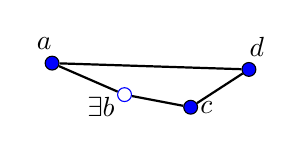
\begin{tikzpicture}
        \node[draw, circle, black, fill=blue, inner sep=0pt, minimum size=5pt,label={[xshift=-0.1cm, yshift=-0.05cm]$a$}] (a) at (0,0) {};
        \node[draw, circle, blue,  inner sep=0pt, minimum size=5pt, label={[xshift=-0.3cm, yshift=-0.5cm]$\exists b$}] (b) at (0.92*1,-0.5*0.8) {};
        \node[draw, circle, black, fill=blue, inner sep=0pt, minimum size=5pt, label={[xshift=0.2cm, yshift=-0.3cm]$c$}] (c) at (1.6*1.1, -0.7*0.8) {};
        \node[draw, circle, black, fill=blue, inner sep=0pt, minimum size=5pt, label={[xshift=0.1cm, yshift=-0.05cm]$d$}] (d) at (2.5*1,-0.2*0.4) {};
    \draw[thick] (a) -- (b) -- (c) -- (d) -- (a);
    \end{tikzpicture}
    \caption{$\vvar_{a,c,d}$}\label{fig:cup}
\end{subfigure}
\hfil
\begin{subfigure}{0.31\textwidth}
    \centering
    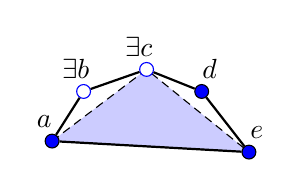
\begin{tikzpicture}
  
    \coordinate (a) at (0,0);
    \coordinate (c) at (1.2*1, 1.3*0.7);
    \coordinate (e) at (2.5*1,-0.2*0.7);
    \fill[blue, opacity=0.2] (a) -- (c) -- (e) -- cycle;
    \draw[densely dashed] (a) -- (c) -- (e) -- (a);

    \node[draw, circle, black, fill=blue, inner sep=0pt, minimum size=5pt,label={[xshift=-0.1cm, yshift=-0.05cm]$a$}] (a) at (0,0) {};
    \node[draw, circle, blue,  fill=white, inner sep=0pt, minimum size=5pt, label={[xshift=-0.1cm, yshift=-0.05cm]$\exists b$}] (b) at (0.4*1,0.9*0.7) {};
    \node[draw, circle, blue, fill=white, inner sep=0pt, minimum size=5pt, label={[xshift=-0.1cm, yshift=-0.05cm]$\exists c$}] (c) at (1.2*1, 1.3*0.7) {};
    \node[draw, circle, black, fill=blue, inner sep=0pt, minimum size=5pt, label={[xshift=0.1cm, yshift=-0.05cm]$d$}] (d) at (1.9*1,0.9*0.7) {};
    \node[draw, circle, black, fill=blue, inner sep=0pt, minimum size=5pt, label={[xshift=0.1cm, yshift=-0.05cm]$e$}] (e) at (2.5*1,-0.2*0.7) {};

    \draw[thick] (a) -- (b) -- (c) -- (d) -- (e) -- (a);
    \end{tikzpicture}
    \caption{$\ufvar_{a,d,e}$}\label{fig:5cap}
\end{subfigure}

\caption{Illustration of the $4$-cap (\ref{fig:cap}), $4$-cup (\ref{fig:cup}), and $5$-cap (\ref{fig:5cap}) variables.  The highlighted region denotes an empty triangle.}\label{fig:cup-cap-vars}
\end{figure}

\begin{figure}
    \centering
    \begin{subfigure}{0.31\textwidth}
        \centering
        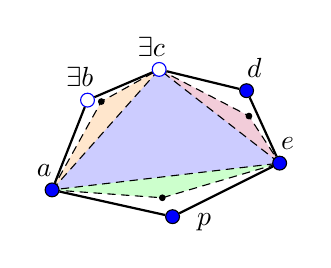
\begin{tikzpicture}
        
    
    
        \coordinate (a) at (0,0);
        \coordinate (c) at (0.8*1.7, 0.9*1.7);
        \coordinate (e) at (1.7*1.7,0.2*1.7);

        \coordinate (p1) at (0.25*2.5, 0.66*1.7);
        \coordinate (p2) at (2.5,0.67*1.4);
        \coordinate (p3) at (1.4,-0.1);

        \fill[blue, opacity=0.2] (a) -- (c) -- (e) -- cycle;
        \fill[orange, opacity=0.2] (a) -- (p1) -- (c) -- cycle;
        \fill[purple, opacity=0.2] (c) -- (p2) -- (e) -- cycle;
        \fill[green, opacity=0.2] (a) -- (p3) -- (e) -- cycle;
        \draw[densely dashed] (a) -- (c) -- (e) -- (a);

        \draw[densely dashed] (a) -- (p1) -- (c);
        \draw[densely dashed] (a) -- (p3) -- (e);
        \draw[densely dashed] (c) -- (p2) -- (e);

        \node[draw, circle, black, fill=blue, inner sep=0pt, minimum size=5pt,label={[xshift=-0.1cm, yshift=-0.05cm]$a$}] (a) at (0,0) {};
        \node[draw, circle, blue, fill=white, inner sep=0pt, minimum size=5pt, label={[xshift=-0.1cm, yshift=-0.05cm]$\exists b$}] (b) at (0.3*1.5,0.6*1.9) {};
        \node[draw, circle, blue, fill=white, inner sep=0pt, minimum size=5pt, label={[xshift=-0.1cm, yshift=-0.05cm]$\exists c$}] (c) at (0.8*1.7, 0.9*1.7) {};
        \node[draw, circle, black, fill=blue, inner sep=0pt, minimum size=5pt, label={[xshift=0.1cm, yshift=-0.05cm]$d$}] (d) at (1.3*1.9,0.7*1.8) {};
        \node[draw, circle, black, fill=blue, inner sep=0pt, minimum size=5pt, label={[xshift=0.1cm, yshift=-0.05cm]$e$}] (e) at (1.7*1.7,0.2*1.7) {};
        \node[draw, circle, black, fill=blue, inner sep=0pt, minimum size=5pt, label={[xshift=0.4cm, yshift=-0.4cm]$p$}] (p) at (0.9*1.7,-0.2*1.7) {};
        \draw[thick] (a) -- (b) -- (c) -- (d) -- (e) -- (p) -- (a);
    
        \node[draw, circle, black, fill=black, inner sep=0pt, minimum size=2pt] (p1) at (0.25*2.5,0.66*1.7) {};
        \node[draw, circle, black, fill=black, inner sep=0pt, minimum size=2pt] (p2) at (2.5,0.67*1.4) {};
        \node[draw, circle, black, fill=black, inner sep=0pt, minimum size=2pt] (p3) at (1.4,-0.1) {};
        \end{tikzpicture}
        \caption{$(\ufvar_{a,d,e} \land \orvar_{a,p,e})$}\label{fig:clause-13-forbid}
    \end{subfigure}
    \hfil
    \begin{subfigure}{0.31\textwidth}
        \centering
        \begin{tikzpicture}
      
       
        \newcommand{\scalefact}{1.3}
        \coordinate (a) at (0*\scalefact,0*\scalefact);
        \coordinate (c) at (0.8*1.7*\scalefact, 0.9*1.7*\scalefact);
        \coordinate (e) at (1.7*1.7*\scalefact,0.2*1.7*\scalefact);

       \coordinate (p1) at (0.25*2.5*\scalefact, 0.66*1.55*\scalefact);
        \coordinate (p2) at (1.8*\scalefact,0.66*1.7*\scalefact);
       \coordinate (bp) at (1.2*\scalefact,0.1*\scalefact);
         \coordinate (cp) at (1.8*\scalefact,0.67*0.8*\scalefact);

        

        \fill[blue, opacity=0.2] (a) -- (c) -- (cp) -- cycle;
        \fill[orange, opacity=0.2] (a) -- (p1) -- (c) -- cycle;
        \fill[purple, opacity=0.2] (c) -- (p2) -- (cp) -- cycle;
       
         \fill[green, opacity=0.2] (a) -- (cp) -- (bp) -- cycle;
    

        \draw[densely dashed] (a) -- (c) -- (cp) -- (a);
        \draw[densely dashed] (a) -- (p1) -- (c);
        \draw[densely dashed] (c) -- (p2) -- (cp);

        \node[draw, circle, black, fill=blue, inner sep=0pt, minimum size=5pt,label={[xshift=-0.1cm, yshift=-0.05cm]$a$}] (a) at (0*\scalefact,0*\scalefact) {};
        \node[draw, circle, blue,  fill=white, inner sep=0pt, minimum size=5pt, label={[xshift=-0.1cm, yshift=-0.05cm]$\exists b$}] (b) at (0.3*1.5*\scalefact,0.6*1.9*\scalefact) {};
        \node[draw, circle, black, fill=blue, inner sep=0pt, minimum size=5pt, label={[xshift=-0.1cm, yshift=-0.05cm]$c$}] (c) at (0.8*1.7*\scalefact, 0.9*1.7*\scalefact) {};
        \node[draw, circle, black, fill=blue, inner sep=0pt, minimum size=5pt, label={[xshift=0.1cm, yshift=-0.05cm]$d$}] (d) at (1.1*1.9*\scalefact,0.7*1.8*\scalefact) {};
        % \node[draw, circle, black, fill=blue, inner sep=0pt, minimum size=5pt, label={[xshift=0.1cm, yshift=-0.05cm]$e$}] (e) at (1.7*1.7,0.2*1.7) {};
        % \node[draw, circle, black, fill=blue, inner sep=0pt, minimum size=5pt, label={[xshift=0.4cm, yshift=-0.4cm]$f$}] (f) at (0.9*1.7,-0.2*1.7) {};
      
    
        \node[draw, circle, black, fill=black, inner sep=0pt, minimum size=2pt] (p1) at (0.25*2.5*\scalefact,0.66*1.55*\scalefact) {};
        \node[draw, circle, black, fill=black, inner sep=0pt, minimum size=2pt] (p2) at (1.8*\scalefact,0.66*1.7*\scalefact) {};

        \node[draw, circle, black, fill=blue, inner sep=0pt, minimum size=5pt, label={[xshift=0.3cm, yshift=-0.2cm]$c'$}] (cp) at (1.8*\scalefact,0.67*0.8*\scalefact) {};
        \node[draw, circle, blue,  fill=white, inner sep=0pt, minimum size=5pt, label={[xshift=0.5cm, yshift=-0.4cm]$\exists b'$}] (bp) at (1.2*\scalefact,0.1*\scalefact) {};

        \draw[thick] (a) -- (b) -- (c) -- (d) -- (cp)  -- (bp) -- (a);
        % \draw[densely dashed] (a) -- (p3) -- (e);
        % \draw[densely dashed] (c) -- (p2) -- (e);
        \end{tikzpicture}
        \caption{$(\uvar_{a,c,d} \land \vvar_{a, c', d} \land \hvar_{a,c,c'})$}\label{fig:clause-14-forbid}
    \end{subfigure}
    \hfil
    \begin{subfigure}{0.31\textwidth}
        \centering
        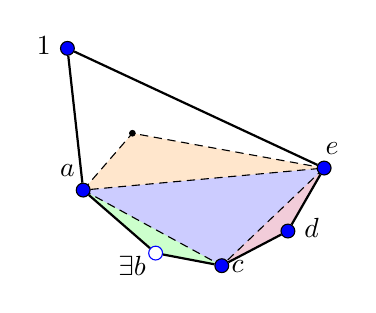
\begin{tikzpicture}
           
        % \node[draw, circle, black, fill=black, inner sep=0pt, minimum size=2pt] (p2) at (2.5,0.67*1.4) {};
        % \node[draw, circle, black, fill=black, inner sep=0pt, minimum size=2pt] (p3) at (1.4,-0.1) {};
    
    
        \coordinate (a) at (0,0.4);
        \coordinate (b) at (0.92*1,-0.5*0.8);
        \coordinate (c) at (1.6*1.1, -0.7*0.8);
        \coordinate (d) at (2.6*1,-0.3*0.4);
        \coordinate (e) at (1.8*1.7,0.4*1.7);

        \coordinate (p1) at (0.25*2.5, 0.66*1.7);
        \coordinate (p2) at (2.5,0.67*1.4);
        \coordinate (p3) at (1.4,-0.1);

        \fill[blue, opacity=0.2] (a) -- (c) -- (e) -- cycle;
         \fill[orange, opacity=0.2] (a) -- (p1) -- (e) -- cycle;
        \fill[purple, opacity=0.2] (c) -- (d) -- (e) -- cycle;
        \fill[green, opacity=0.2] (a) -- (b) -- (c) -- cycle;
        % \draw[densely dashed] (a) -- (c) -- (e) -- (a);


         \draw[densely dashed] (a) -- (c) -- (e) -- (a);

       
        \draw[densely dashed] (a) -- (p1) -- (e);

        \node[draw, circle, black, fill=blue, inner sep=0pt, minimum size=5pt,label={[xshift=-0.2cm, yshift=-0.05cm]$a$}] (a) at (0,0.4) {};
        \node[draw, circle, blue,  fill=white, inner sep=0pt, minimum size=5pt, label={[xshift=-0.3cm, yshift=-0.5cm]$\exists b$}] (b) at (0.92*1,-0.5*0.8) {};
        \node[draw, circle, black, fill=blue, inner sep=0pt, minimum size=5pt, label={[xshift=0.2cm, yshift=-0.3cm]$c$}] (c) at (1.6*1.1, -0.7*0.8) {};
        \node[draw, circle, black, fill=blue, inner sep=0pt, minimum size=5pt, label={[xshift=0.3cm, yshift=-0.3cm]$d$}] (d) at (2.6*1,-0.3*0.4) {};
        \node[draw, circle, black, fill=blue, inner sep=0pt, minimum size=5pt, label={[xshift=-0.3cm, yshift=-0.3cm]$1$}] (1) at (-0.2*1,2.2) {};
        

    % \node[draw, circle, black, fill=blue, inner sep=0pt, minimum size=5pt,label={[xshift=-0.1cm, yshift=-0.05cm]$a$}] (a) at (0,0) {};
    % \node[draw, circle, blue,  inner sep=0pt, minimum size=5pt, label={[xshift=-0.1cm, yshift=-0.05cm]$\exists b$}] (b) at (0.3*1.5,0.6*1.9) {};
    % \node[draw, circle, blue, inner sep=0pt, minimum size=5pt, label={[xshift=-0.1cm, yshift=-0.05cm]$\exists c$}] (c) at (0.8*1.7, 0.9*1.7) {};
    % \node[draw, circle, black, fill=blue, inner sep=0pt, minimum size=5pt, label={[xshift=0.1cm, yshift=-0.05cm]$d$}] (d) at (1.3*1.9,0.7*1.8) {};
    \node[draw, circle, black, fill=blue, inner sep=0pt, minimum size=5pt, label={[xshift=0.1cm, yshift=-0.05cm]$e$}] (e) at (1.8*1.7,0.4*1.7) {};
    % \node[draw, circle, black, fill=blue, inner sep=0pt, minimum size=5pt, label={[xshift=0.4cm, yshift=-0.4cm]$f$}] (f) at (0.9*1.7,-0.2*1.7) {};
    % \draw[thick] (a) -- (b) -- (c) -- (d) -- (e) -- (f) -- (a);

 \node[draw, circle, black, fill=black, inner sep=0pt, minimum size=2pt] (p1) at (0.25*2.5,0.66*1.7) {};
 \draw[thick] (1) -- (a) -- (b) -- (c) -- (d) -- (e) -- (1);
        % \draw[densely dashed] (c) -- (p2) -- (e);
        \end{tikzpicture}
        \caption{$(\vvar_{a,c,d} \land \orvar_{c, d, e} \land \hvar_{a,c,e})$}\label{fig:clause-15-forbid}
    \end{subfigure}
    \caption{Illustration of some \emph{forbidden configurations} that imply $6$-holes. \Cref{fig:clause-13-forbid} corresponds to the configuration forbidden by clause~\labelcref{eq:no6Hole1Below}, \Cref{fig:clause-14-forbid} to the one forbidden by clause~\labelcref{eq:no6Hole2Below1}, and~\Cref{fig:clause-15-forbid} to clause~\labelcref{eq:no6Hole3Below}. All highlighted regions denote empty triangles.}\label{fig:forbidden}
\end{figure}
